\section[COVID-19]{Let's talk about COVID-19}
\stepcounter{subsection} %We don't use subsection titles, only frametitles
\label{sec:covid}

%---------------------------------------------------------------
% 1. Why do we want to talk about COVID-19?
%---------------------------------------------------------------
\begin{frame}{Why would we want to talk about COVID-19?}

\begin{columns}[c]
    \begin{column}{0.45\textwidth}
    
        COVID-19 is...
        
        \begin{itemize}
            \item something we've all experienced,
            \item international, and
            \item recent,
        \end{itemize}
            
        ... and a great example of how we experience and share science!
    \end{column}
        
    \begin{column}{0.45\textwidth}
        \centering
        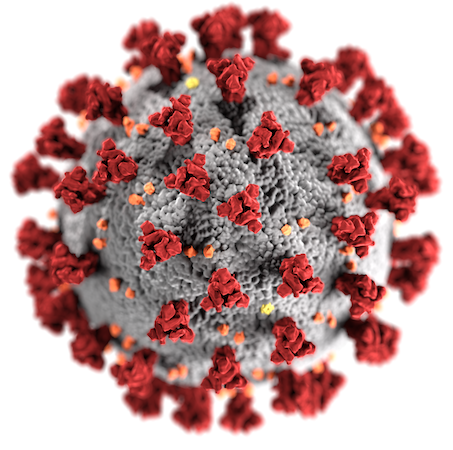
\includegraphics[width=0.8\textwidth]{images/PHIL_23312_lowres.png}\\
        \simplecaption{\centering The SARS-CoV-2 Virus}
        \givecredit{\centering Source: \textlink{https://phil.cdc.gov/Details.aspx?pid=23312}{Public Health Image Library \#23312}.\\
        Credit: Alissa Eckert, MSMI, Dan Higgins, MAMS.}
    \end{column}

\end{columns}

\end{frame}

%---------------------------------------------------------------
% 2. How we learned about COVID-19
%---------------------------------------------------------------

\begin{frame}{How did we learn about COVID-19?}

\begin{columns}[t]
    % sources of information
    \column{.45\textwidth}
    \begin{block}{Mainstream media}
        \begin{itemize}
            \item Traditional news
            \item Social media
        \end{itemize}
    \end{block}
    
    \begin{block}{Scientific media}
        \begin{itemize}
            \item Researchers' websites
            \item Paper repositories
        \end{itemize}
    \end{block}
    
     \begin{block}{Personal experience}
        \begin{itemize}
            \item Directly affected
            \item Rumours and gossip
        \end{itemize}
    \end{block}
    
    % discussion points
    \column{.45\textwidth}

    What do you think?

    \begin{itemize}
        \item What makes information useful?
        \item What makes you take action?
        \item What can we learn from this?
    \end{itemize}
        
\end{columns}    

\end{frame}

%---------------------------------------------------------------
% 3. How people responded
%---------------------------------------------------------------

\begin{frame}{How did we respond to COVID-19?}

\centering
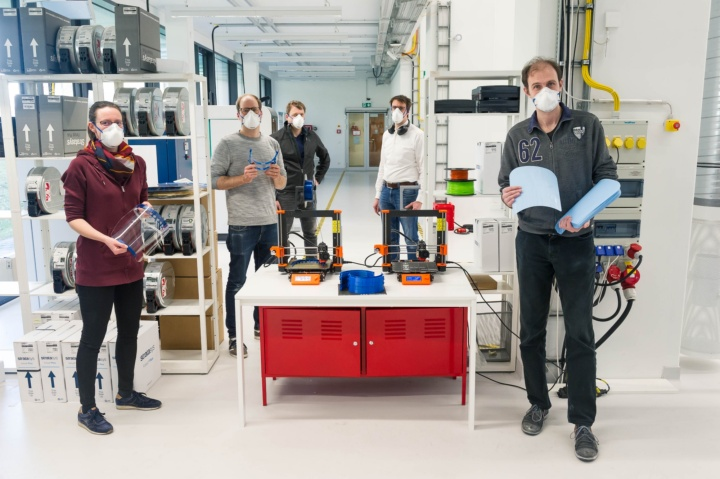
\includegraphics[width=0.7\textwidth]{images/2020_04_02_Maske_002.jpg}\\

\simplecaption{\centering The ARENA2036 team and many others made face shields to protect against coronavirus. Source: \textlink{https://www.uni-stuttgart.de/en/university/news/press-release/The-University-of-Stuttgart-shows-solidarity-with-hospitals-and-medical-practices-in-the-region-in-the-fight-against-coronavirus-infections/}{U. Stuttgart}}

\end{frame}

%---------------------------------------------------------------
% 4. It didn't always work well
%---------------------------------------------------------------

\begin{frame}{How was scientific information shared?}

\centering
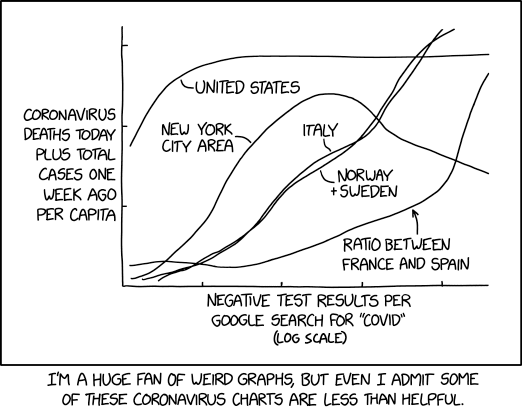
\includegraphics[width=0.6\textwidth]{images/xkcd_2294.png}\\

\givecredit{\centering Source: \textlink{https://xkcd.com/2294/}{xkcd}}

\end{frame}

%---------------------------------------------------------------
% 5. Lessons we can learn
%---------------------------------------------------------------

\begin{frame}{Lessons learned from COVID-19}

\begin{columns}[t]
    % lessons
    \begin{column}{.5\textwidth}   
        Openness has advantages:
        
        \begin{itemize}
            \item Monitoring spread of the SARS-CoV-2 virus
            \item Sharing treatment plans across continents
            \item Developing technical solutions
        \end{itemize}

    \vspace{1cm}

        But it brings new challenges for STEM experts:

        \begin{itemize}
            \item Communicating (uncertain) results
            \item Making scientific information useful
        \end{itemize}
    \end{column}

    \begin{column}{.4\textwidth}
        \vspace{-1cm}
    
        \centering
        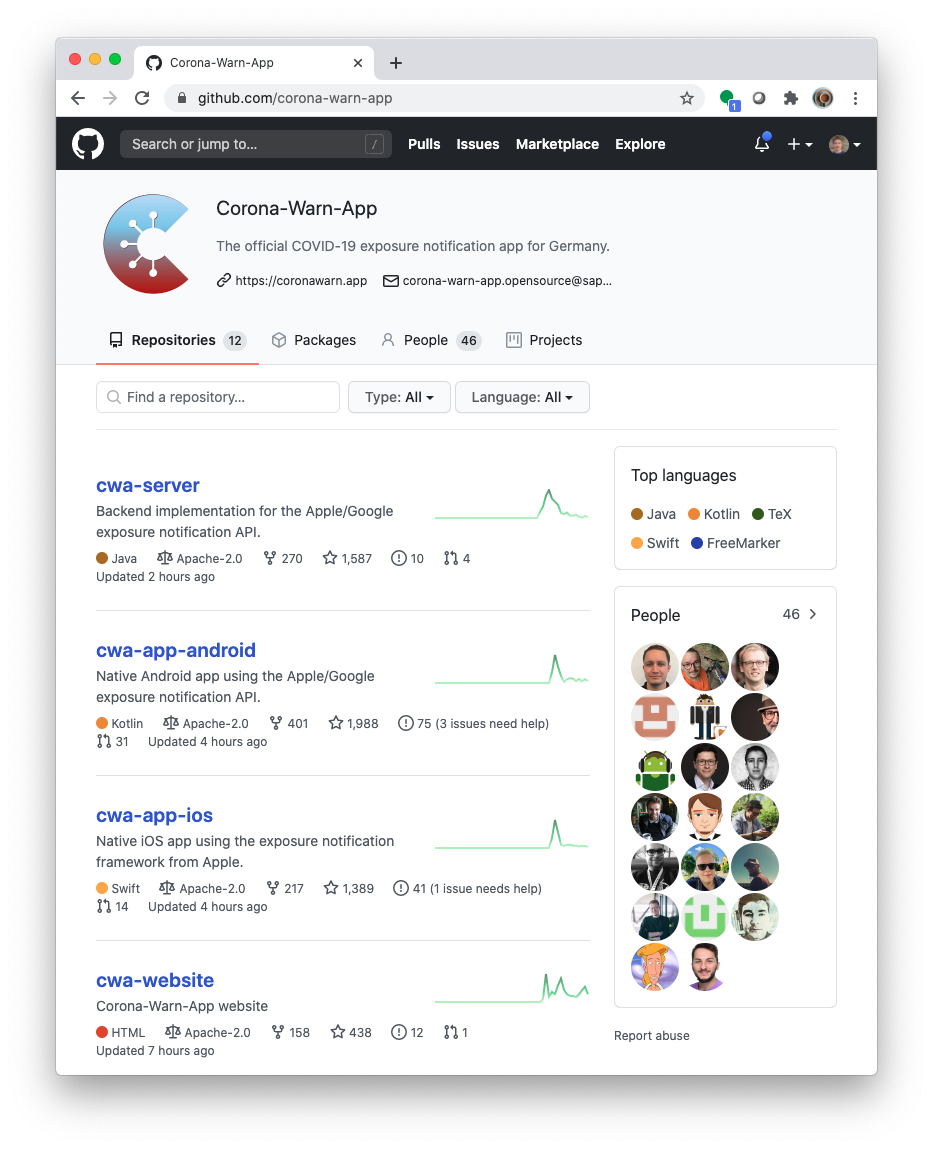
\includegraphics[width=\textwidth]{images/Corona-warn-app.png}\\
        
        \simplecaption{\centering%
        The German COVID-19 exposure notification app source code is shared through \textlink{https://github.com/corona-warn-app}{GitHub}}
        \label{fig:my_label}
    \end{column}
    

\end{columns}

\end{frame}